% ==================== GUIDA ALL'UTILIZZO ==========================================

\newpage

\enlargethispage{1\linewidth}

\section{Guida all'Utilizzo}

\textsf{\small Qui, di seguito verranno indicate le procedure e le istruzioni da eseguire per poter avviare correttamente il programma: } \\

\begin{itemize}
	\item \textsf{\small Caricare il file \emph{aeroportoDbCreation} nella directory \emph{db} su \textbf{MySQL} ed eseguirlo.}
	\item \textsf{\small Dopo aver creato il database con successo, allora eseguire il file \emph{aeroportoDbData} per caricare i dati su cui poter lavorare.}
	\item \textsf{\small Aprire il file, la classe java \textbf{Database} nella directory \emph{src/main/java/com/lucar01/aeroporto/Database.java} (Immagine: \ref{fig:database}) e lì sarà possibile modificare i seguenti parametri che riguardano l'accesso al database su \textbf{MySQL}: }
	\begin{itemize}
		\item \textsf{\small \emph{databaseUser} : di default è impostato su \textbf{root}, ma è possibile cambiarlo se si vuole utilizzare un altro utente.}
		\item \textsf{\small \emph{databasePassword} : impostata, di default, su \textbf{" "}, ma è possibile cambiarla se si utilizza una password differente.}
	\end{itemize}
	\item \textsf{\small Per quanto riguarda le altre variabili non dovrebbe essere necessario modificarle, visto che il nome del database è quello già impostato, ovvero \emph{aeroporto} e l'url dovrebbe anch'esso essere corretto.}
	\item \textsf{\small Dopodichè eseguire il \textbf{Main.java} e la schermata dell'applicativo dovrà apparire.}
\end{itemize}

\begin{figure}[ht] 
	\centering
	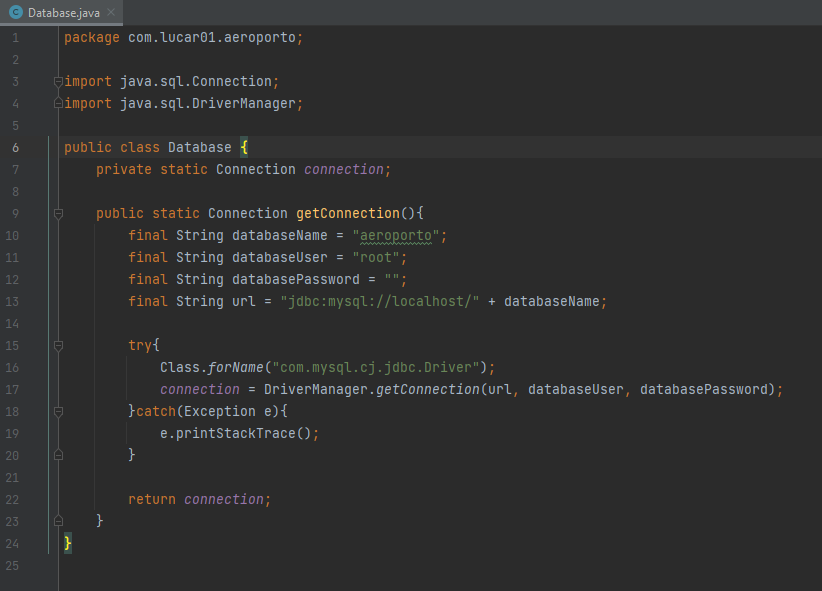
\includegraphics[width=1\textwidth, height=1\textheight, keepaspectratio]{./img/Applicativo/database_class.png}
	\caption{Classe Database}
	\label{fig:database}
\end{figure}
